\documentclass[12pt,twoside,english,a4paper]{article}

\usepackage[english]{babel}
\usepackage[IL2]{fontenc} % lepšia sadzba písmena Ľ než v T1
\usepackage[utf8]{inputenc}
\usepackage{graphicx}
\usepackage{url} % príkaz \url na formátovanie URL
\usepackage{hyperref} % odkazy v texte budú aktívne (pri niektorých triedach dokumentov spôsobuje posun textu)

\usepackage{cite}
%\usepackage{times}

\pagestyle{headings}

\title{FOOTBAL SIMULATORS (FIFA AND PES)}

\author{Dmytro Barninets\\[2pt]
	{\small Slovenská technická univerzita v Bratislave}\\
	{\small Fakulta informatiky a informačných technológií}\\
	{\large \texttt{xbarninets@stuba.sk}}
	}

\date{\large 11. october 2022}



\begin{document}

\maketitle


\section{Why did i chose this topic?} \label{mainparagraph}

The main reason I chose this theme is the popularity of football games. Among sports simulators, it is FIFA that occupies a leading position in online.


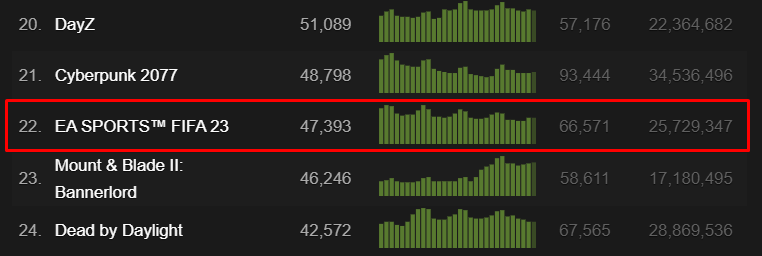
\includegraphics[width=150mm,scale=1.5]{fifa_charts.png} \label{chartsphoto}


As of November 4, an average of 47,000 players play FIFA. And this is only in Steam, excluding consoles and less popular game launchers.


As for PES, the situation with online is much worse at the moment \emph{(more on that later)}. But that doesn't stop footsim fans from remembering this series as legendary.

In general, football simulators are not as simple and monotonous as at first glance.

\section{Differences between FIFA and PES} \label{differences}\cite{Gaming.net}

\begin{itemize}
\item What is FIFA?

FIFA is a video game series that is published by Electronic Arts (EA) and developed by EA Canada.

From the very first versions FIFA obtained more licenses in comparison to their rivals. The licenses obtained include permits for stadiums, players and their respective clubs. This helps guarantee the production of realistic football games; since users prefer playing with real characters, they are familiar with and can relate to. That and various other aspects are what make FIFA a remarkable series. In terms of sales, FIFA is ahead of PES, although the latter has always been regarded as the better game. Nonetheless, it may still have a long way to go before it achieves the same commercial effect as FIFA.

\item What is PES?

Pro Evolution Soccer [PES] is a video game series that is published by Konami and developed by PES Productions. PES games are released annually, with the latest one being PES 2021. 

Much like FIFA, PES aspires to be as realistic as possible when it comes to depicting real-life football. Hence, the gameplay in its series is identical to association soccer, whereby players control either one player or a whole team. The ideas of the game also correspond with the rules and regulations of the football association.
	
\end{itemize}

The most apparent difference between the two game brands is the time gap between the first launch of PES’s first game and that of FIFA. This gave FIFA a chance to fully develop a fan base and perfect its products over the years. 

However, PES was able to compete as they adopted much more diverse models in their gameplay compared to FIFA. Similarly, in terms of gameplay, most fans regard PES as more practical, whilst FIFA is considered more refined in design and presentation. 




\section{Game aspects} \label{aspects}




\subsection{Graphics} \label{aspects: graphics}

\subsection{Gameplay} \label{aspects: gameplay}

\subsection{Game modes} \label{aspects: modes}

\subsection{Teams} \label{aspects: teams}

\subsection{Players} \label{aspects: players}

Niekedy treba uviesť zoznam:

\begin{itemize}
\item jedna vec
\item druhá vec
	\begin{itemize}
	\item x
	\item y
	\end{itemize}
\end{itemize}

Ten istý zoznam, len číslovaný:

\begin{enumerate}
\item jedna vec
\item druhá vec
	\begin{enumerate}
	\item x
	\item y
	\end{enumerate}
\end{enumerate}


\bibliography{literatura}
\bibliographystyle{plain}
\end{document}
